%%%%%%%%%%%%%%%%%%%%%%%%%%%%%%%%%%%%%%%%%%%%%%%%%%%%%%%%%%%%%%
\chapter{Observed Truck-Visit Behaviour}
\label{app:observed_behaviour}
%%%%%%%%%%%%%%%%%%%%%%%%%%%%%%%%%%%%%%%%%%%%%%%%%%%%%%%%%%%%%%
% Moved from Chapter 4 (Data Preparation) on 5 Nov 2026.
% Source: trucksimulation/peak_analysis/peak_analysis_observed_v2.py,
% output peak_analysis/observed_20261007_v2. Training and validation only.

This appendix describes the recorded behaviour that the simulation must
reproduce, in more detail than Section~\ref{sec:observed_behaviour}. All
statements are descriptive associations. They do not establish causes.
Thresholds are fitted on the training partition and applied unchanged to the
validation partition. The test partition is not used.

\section{Arrival Pattern}
\label{sec:obs_arrivals}

Trucks arrive in a stable weekly and daily pattern
(Figure~\ref{fig:obs_calendar}). Arrivals take place from Monday to
Friday, with few visits on Saturdays and none on Sundays. On weekdays,
about 22 trucks per hour arrive between midnight and 5:00. The rate
rises to about 118 per hour at 6:00 and stays on a plateau of 126 to 152
trucks per hour between 7:00 and 16:00. After 17:00 it falls again. The
week around Easter (1 to 7 April) has a markedly lower volume.

An \emph{arrival peak} is a Gate-In hour with at least 165 arrivals, the
90th percentile of all training hours with arrivals. Arrival peaks are
short spikes on top of the daytime plateau. They make up 70 of 610
training hours with at least 20 visits (11.5\,\%) and 18 of 147
validation hours. The highest hourly count is 255 trucks, in the
validation period.

\begin{figure}[htbp]
\centering
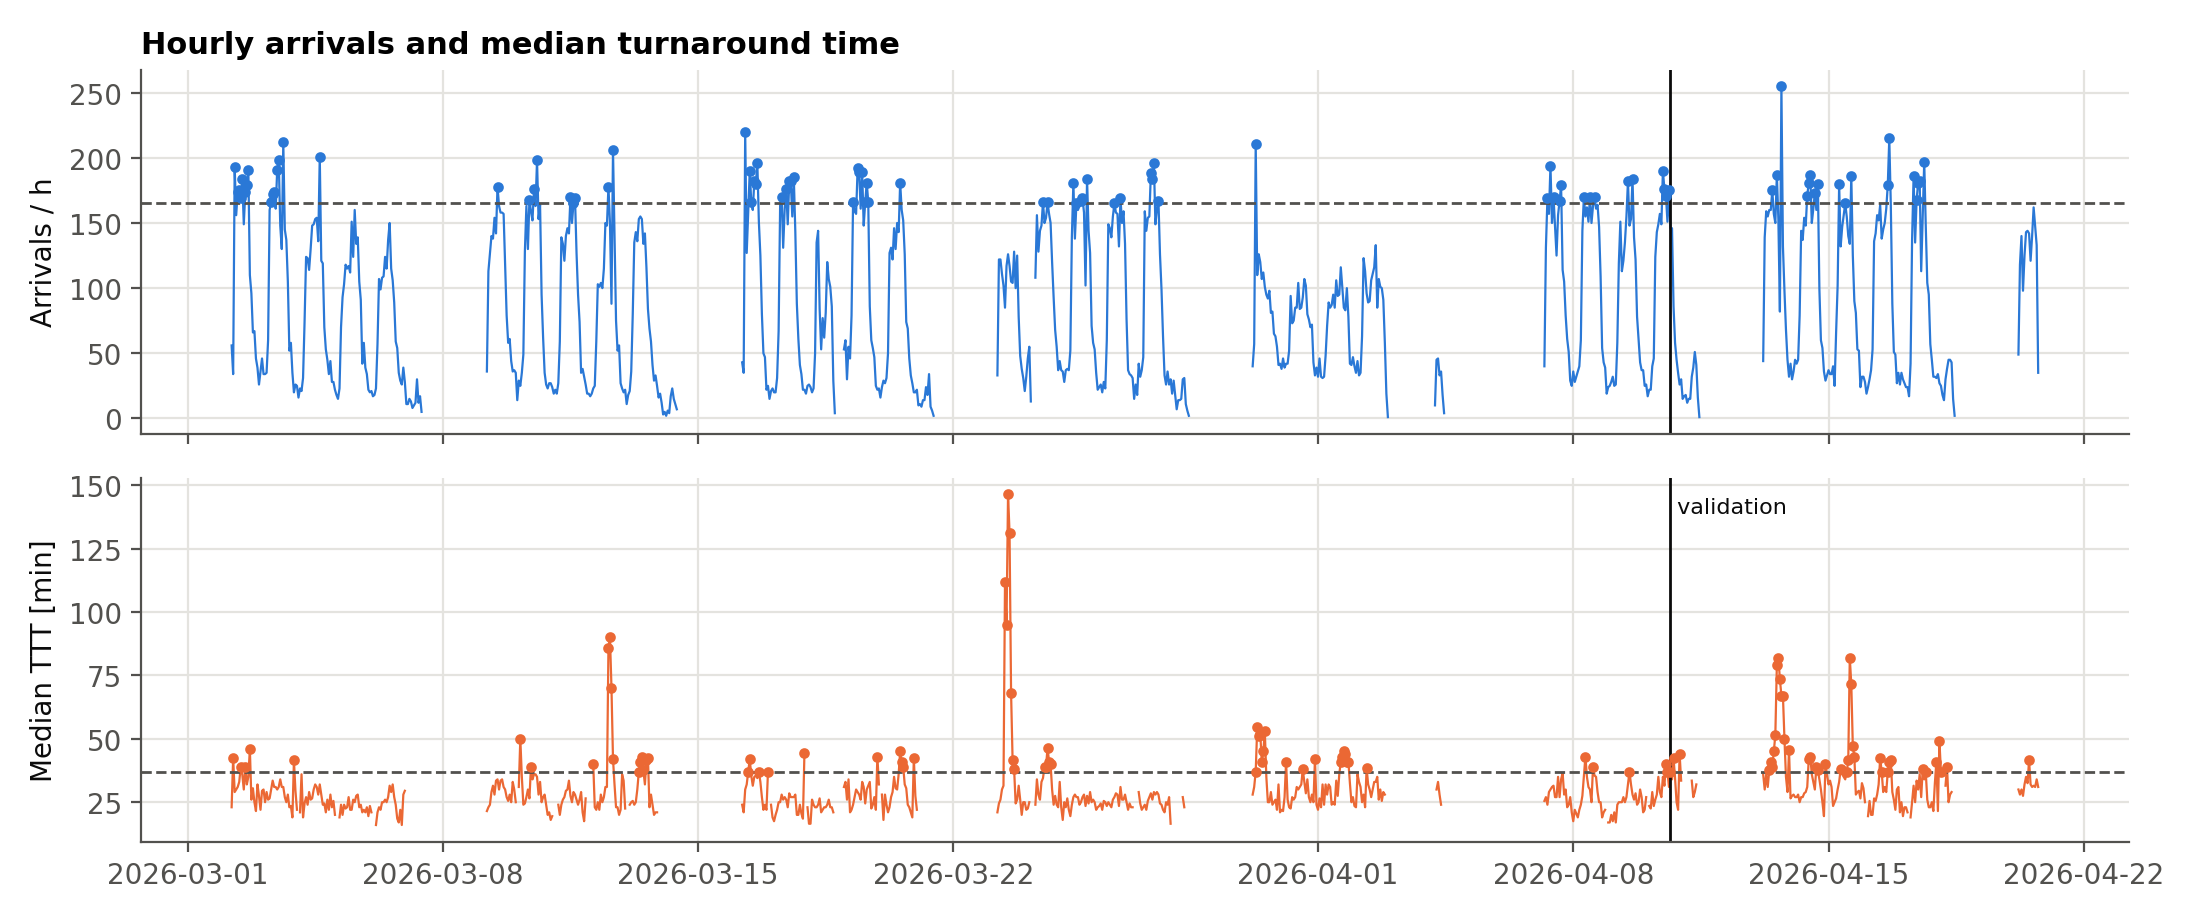
\includegraphics[width=\textwidth]{figures/observed/hourly_arrivals_ttt.png}
\caption{Hourly arrivals (top) and median turnaround time by Gate-In hour
(bottom) for the training and validation periods. Dots mark arrival peaks
and delay peaks. Dashed lines show the thresholds of 165 arrivals and
37 minutes. The vertical line marks the start of the validation period.}
\label{fig:obs_calendar}
\end{figure}

\section{Congestion over the Day}
\label{sec:obs_congestion}

The turnaround time grows over the working day, although the arrival
rate stays on its plateau. On training weekdays, the median TTT rises
from 26 minutes for trucks arriving at 7:00 to 34 minutes at 14:00. The
P90 rises from 57 to 81 minutes at 13:00. The mean number of trucks
already inside the terminal at Gate In grows from 69 at 7:00 to 106 at
15:00. Figure~\ref{fig:obs_components} shows that this growth comes mainly
from the approach and the exit. The stop intervals change comparatively
little over the day.

\begin{figure}[htbp]
\centering
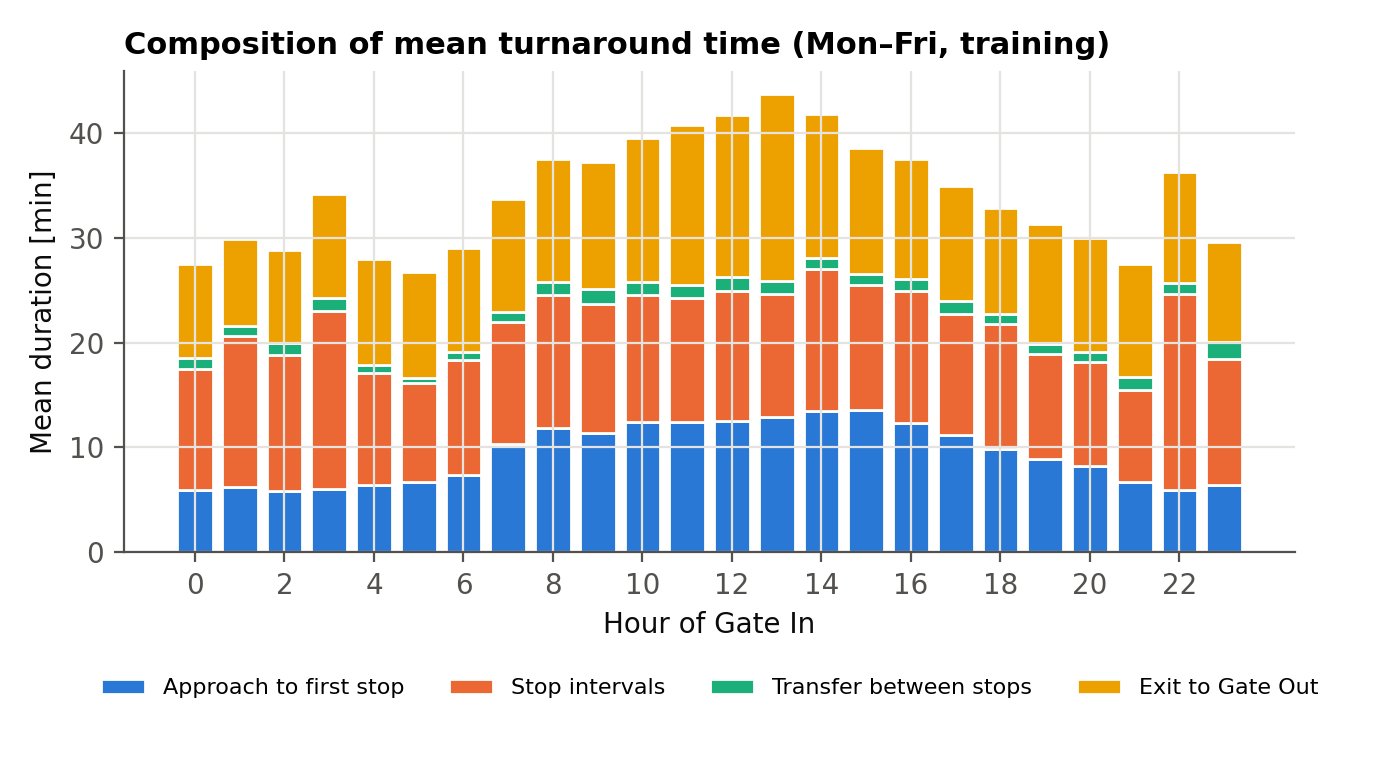
\includegraphics[width=0.85\textwidth]{figures/observed/ttt_components_by_hour.png}
\caption{Mean turnaround time by Gate-In hour, split into approach, stop
intervals, transfer and exit. Training weekdays.}
\label{fig:obs_components}
\end{figure}

The turnaround time increases with the number of trucks in the terminal,
and the increase is non-linear (Figure~\ref{fig:obs_wip}). Up to about
100 trucks, the median TTT rises slowly from 23 to 34 minutes. Between
140 and 160 trucks, the median reaches 43 minutes and the P90 about 100
minutes. Above 160 trucks, the P90 exceeds two hours. Such occupancy
levels are rare and occur on a few days only. The
Spearman correlation between hourly arrivals and the median TTT of the
same hour is 0.51. It is 0.53 for the arrivals of the preceding three
hours and drops to 0.05 for a lag of six hours.

\begin{figure}[htbp]
\centering
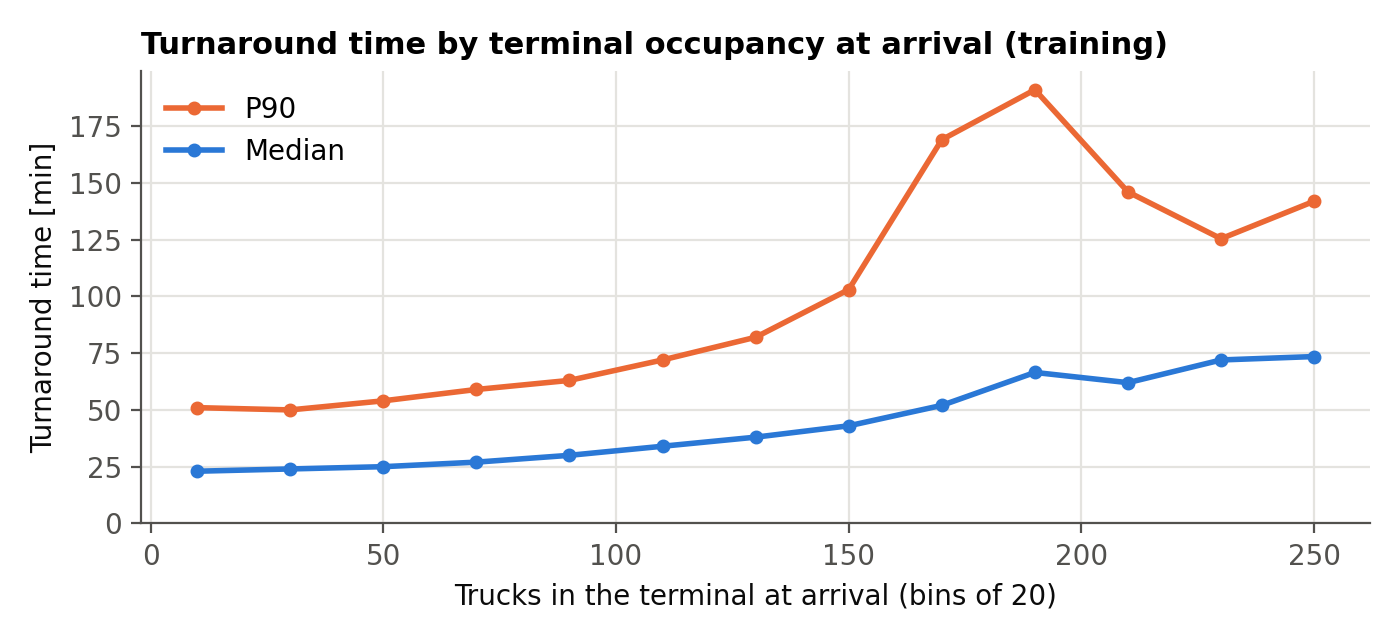
\includegraphics[width=0.85\textwidth]{figures/observed/ttt_vs_wip.png}
\caption{Median and P90 of the turnaround time by the number of trucks
in the terminal at Gate In, in classes of 20. Training, classes with at
least 50 visits.}
\label{fig:obs_wip}
\end{figure}

The same pattern appears at the handling units
(Figure~\ref{fig:obs_unit}). At an RMG block, the median stop interval
is 5 minutes when the truck is alone at the block. It is 9, 13 and 18
minutes when two, three or four trucks have an open interval at the same
block. The Spearman correlation between unit occupancy and stop duration
is 0.49 for RMG, 0.45 for LL and 0.32 for HO2. Up to four concurrent
intervals occur at an RMG block, although a block has three handover
lanes. How a fourth interval arises is not yet clear. At LL and HO2,
more than ten concurrent intervals occur. This confirms that the
timestamps of these areas do not represent physical occupancy.

\begin{figure}[htbp]
\centering
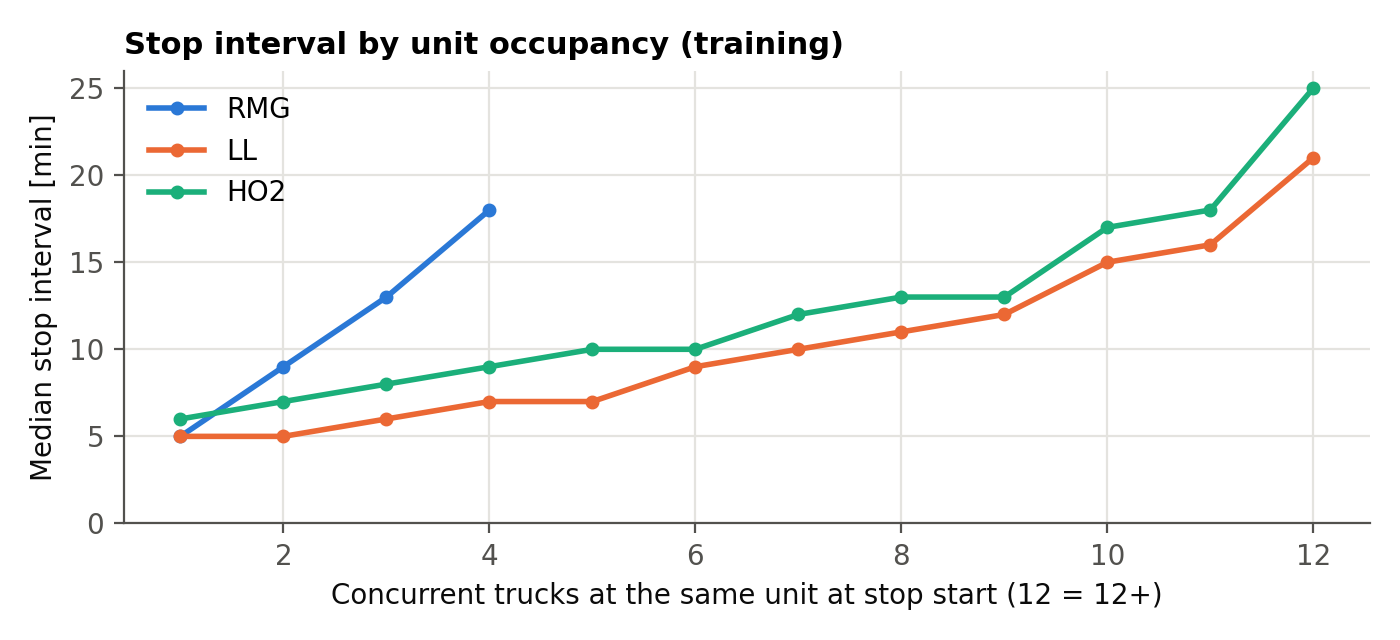
\includegraphics[width=0.85\textwidth]{figures/observed/stop_vs_unit_wip.png}
\caption{Median stop interval by the number of trucks with an open
interval at the same handling unit when the stop starts. Training.}
\label{fig:obs_unit}
\end{figure}

\section{Delay Peaks}
\label{sec:obs_delay_peaks}

A \emph{delay peak} is a Gate-In hour with at least 20 visits whose
median TTT is at least 37 minutes, the 90th percentile of the training
hours. Delay peaks are a different phenomenon from arrival peaks.
Training contains 62 delay-peak hours (10.2\,\%) and validation 39
(26.5\,\%). Only nine delay-peak hours in each partition are also
arrival-peak hours.

Table~\ref{tab:obs_peak_components} decomposes the turnaround time in
and outside delay peaks. In training, the mean TTT in delay-peak hours
is 24.4 minutes longer. Approach and exit account for 21.4 minutes of
this difference, or 88\,\%. The stop intervals grow by only 2.5 minutes.
Arrival peaks, in contrast, are associated with an increase of only 2.4
minutes in mean TTT.

The exit share is driven by two disruption days
(Section~\ref{sec:obs_episodes}). Without 12 and 23 March, the mean TTT
in delay-peak hours is 17.0 minutes longer. The approach accounts for
10.1 minutes (59\,\%), the stop intervals for 3.3 minutes (19\,\%) and
the exit for 3.1 minutes (18\,\%). Under normal operation, the additional
delay therefore arises mainly before the truck reports ready at its
first stop.
% Source: peak_analysis/bottleneck_analysis.py, output bottleneck_20261009.

\begin{table}[htbp]
\centering
\begin{tabularx}{\textwidth}{YL{1.5cm}L{1.5cm}L{1.5cm}L{1.5cm}L{1.5cm}}
\toprule
\textbf{Training, mean [min]} & \textbf{Approach} & \textbf{Stops} & \textbf{Transfer} & \textbf{Exit} & \textbf{TTT} \\
\midrule
Delay-peak hours (7,273 visits) & 19.3 & 14.2 & 1.6 & 22.9 & 57.9 \\
Other hours (50,989 visits) & 9.8 & 11.7 & 1.1 & 11.0 & 33.5 \\
Difference & +9.5 & +2.5 & +0.5 & +11.9 & +24.4 \\
\midrule
Arrival-peak hours (12,732 visits) & 12.0 & 12.4 & 1.2 & 12.9 & 38.4 \\
Other hours (45,530 visits) & 10.7 & 11.9 & 1.1 & 12.3 & 36.0 \\
\bottomrule
\end{tabularx}
\caption{Turnaround-time components in and outside peak hours. Visits
are assigned to the hour of their Gate In.}
\label{tab:obs_peak_components}
\end{table}

Not all visits are affected equally. In arrival peaks, the median TTT of
receive visits rises from 28 to 34 minutes, that of delivery visits only
from 23 to 25 minutes. Multiblock visits rise from 45 to 52 minutes.
Visits without RMG are almost unaffected (27 to 28 minutes). Among the
RMG blocks, T18 shows the largest increase of the median stop interval,
from 10 to 17 minutes. Most other blocks increase by at most three
minutes, and HO2 stops are not longer in arrival peaks.

\section{Disruption Episodes}
\label{sec:obs_episodes}

A few delay peaks follow a different pattern. On Monday, 23 March 2026,
the hourly median TTT rose to between 112 and 146 minutes from about
9:30, while arrivals stayed at a normal 85 to 126 trucks per hour. Up to
306 trucks were inside the terminal. The additional time lies almost
entirely in the exit, with approach and stop intervals at normal values.
Similar but shorter episodes occur on 12 March and on 13 April
(validation). Possible explanations include a disruption at the exit
gate or in exit processing, or an artefact of the Gate Out recording.
% TODO: add the explanation from the domain review (questionnaire D9).
Such episodes are not driven by demand. A simulation learned from normal
operations cannot be expected to reproduce them. They are therefore
identified by a rule fixed in advance and reported separately, but they
are never removed from the evaluation.

\section{Differences between the Partitions}
\label{sec:obs_drift}

The validation period is more congested than the training period
(Table~\ref{tab:obs_drift}). Its daily median TTT is 32 minutes against
29, and the share of delay-peak hours is 26.5\,\% against 10.2\,\%.
Visits without RMG show the largest shift, with a median TTT of 39
against 27 minutes. The mix of visits shifts as well: the validation
period has more deliveries, more visits without RMG and more visits with
two or more stops.

\begin{table}[htbp]
\centering
\begin{tabularx}{\textwidth}{YL{3.2cm}L{3.2cm}}
\toprule
\textbf{Measure} & \textbf{Training} & \textbf{Validation} \\
\midrule
Visits & 58,262 & 14,625 \\
TTT mean / median / P90 [min] & 36.5 / 28.5 / 64 & 42.2 / 34 / 78 \\
Daily median TTT [min] & 29 & 32 \\
Mean approach / exit [min] & 10.9 / 12.5 & 13.2 / 13.6 \\
Delay-peak hours (of operating hours) & 10.2\,\% & 26.5\,\% \\
Visits without RMG: share, median TTT & 22.5\,\%, 27 min & 27.1\,\%, 39 min \\
Delivery / receive / mixed visits & 38.6 / 48.2 / 13.2\,\% & 42.2 / 43.4 / 14.5\,\% \\
Visits with two or more stops & 8.7\,\% & 10.2\,\% \\
\bottomrule
\end{tabularx}
\caption{Observed visits per partition. Delay-peak threshold (37
minutes) fixed on the training period.}
\label{tab:obs_drift}
\end{table}

The shift affects the frequencies of activity sequences rather than
their set. Only six validation visits (0.04\,\%) follow a sequence that
does not occur in training, each a different one. The
control-flow log distance between equal-size samples of training visits
and the validation log is 0.024 to 0.027, and 0.036 for the last 14,625
training visits. The distance between their turnaround-time
distributions is 6.3 to 6.6 minutes (Section~\ref{sec:res_baseline}
uses the same measures for the generated logs).
% Source: trucksimulation/simulation_e3/runs/conformance_20261011 (reference rows).

A model fitted on the training period is therefore expected to
underestimate the validation TTT, independently of its control flow.
Errors measured on the validation period mix model error and drift. Two
references separate them. A replay of the training period with the
fitted model measures the model error without drift. The distance
between two real periods shows how close any model fitted on one period
can be to another. In addition, model variants are compared with each
other on the same period.

\section{Bottlenecks at the Handover}
\label{sec:obs_bottlenecks}
\begin{hints}
\item Evidence used by scenario S1: approach to the first RMG stop by trucks already at the block at Gate In (median 6, 6, 9, 14, 20 min for 0--4 trucks); stop duration growth by block (T18 6 to 19 min); in 11\,\% of arrivals the target block is full while a median of 14 other blocks have at most one truck; exit gate not a bottleneck in normal operation (source: peak\_analysis/bottleneck\_20261009, scenario\_evidence.py).
\end{hints}
